\newpage
\section{How to use mesh topologies in SOFA}

H. Delingette, B. Andr�

\subsection{Introduction}

\subsubsection{BTW, What is a mesh topology ?}

A mesh is usually described as a set of points that are connected by
edges, triangles or any other type of mesh element. Thus it is
useful to make a clear a distinction between two different aspects
of a mesh :

\begin{itemize}

 \item \textbf{Mesh Geometry} : the mesh geometry consists in the position of the mesh vertices.
This information depends on the space where the mesh in embedded.
For instance in a 2D triangulation, each vertex position is a 2D
vector while in a 3D triangulation, each vertex position is a 3D
vector. Therefore the mesh geometry can be described as an array of
vector whose size is the number of mesh vertices. In SOFA, we use
the word Degree Of Freedom (DOF) to describe such an array because
it can be used to store other geometric information (rigid
transformation, first or second derivatives, etc.).

 \item \textbf{Mesh Topology} : the mesh topology describes how the vertices are
connected with each other. For instance, it describes the set of
triangles by specifying the 3 vertex indices that make each
triangle. A mesh topology manipulates vertex indices (as unsigned
int) and therefore is independent of the embedding space. For
instance, a 2D and a 3D triangulation may have the same mesh
topology but with different mesh geometry.

\end{itemize}


\subsubsection{Why do I need to bother with mesh topologies ?}

As discuss above, mesh topology is an essential part of a mesh and
therefore any computation task that requires a mesh needs to know
how to use a mesh topology.\\ This includes:

\begin{itemize}

 \item \textbf{Mesh Visualization},

 \item \textbf{Collision detection} : some collision detection are mesh based (e.g.
triangles or edges),

 \item \textbf{Mechanical Modeling} : deforming a mesh also requires to the
knowledge of a mesh topology. For instance a spring mass model
requires knowing about the edges that connects pair of vertices,

 \item \textbf{Haptic rendering},

 \item \textbf{Description of scalar} (temperature, electric potential, etc.) or
vectorial fields (speed, fiber orientation, etc.)

\end{itemize}

Using a mesh topology is relatively simple since it consists in
having access to arrays of indices corresponding to vertex indices
or edge indices or other topological items.
\\

A more tricky part consists a) in changing locally or globally this
topology (adding a triangle, removing an edge) and b) in propagating
those changes to all objects using the mesh topology to perform a
task (visualization, deformation, etc.)

\subsubsection{How are Mesh Topologies designed in SOFA ?}

The mesh geometry in SOFA is stored in a MechanicalObject which is a
template class because it depends on the embedding space (2D or 3D
Euclidian space), the vector class and the required floating point
accuracy (float vs double).
\\

A mesh topology is stored in a different object than the mesh
geometry.
\\

One important aspect of the design of mesh topologies in SOFA is the
fact that they are organized in a class hierarchy. For instance, a
triangulation object derives from an edge set object since a
triangulation can be also viewed as a set of edges, each triangle
having 3 edges. This is very important to design generic software
components. Indeed, following the same example, with this design, a
spring mass mechanical model that only requires the knowledge of
edges (pairs of vertices) can also be used on a triangulation or any
other mesh (quad, hexahedral, tetrahedral mesh)  that derives from
an edge set object.
\\

Another interesting feature in SOFA is the ability to provide
multiple topology descriptions for the same mesh. For instance a
quad element (see figure below) has four DOFs which can be connected
with 2 triangles or 6 edges. Thus, the same mesh geometry can be
described by 3 different mesh topologies. SOFA uses the mechanism of
topological mapping to provide multiple topologies associated with
the same mesh geometry. Those mappings also apply to map a subset of
the mesh topology into a new mesh topology.  For instance the border
of a tetrahedral mesh can be mapped into triangulation mesh or edges
of a triangulated mesh can be mapped into a polygonal mesh.\\


\begin{figure*}
 \centering
 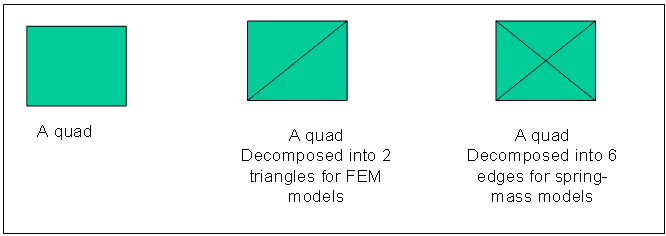
\includegraphics[width=0.95\linewidth]{Quad_Multiple_Topologies}
  \caption{Multiple topology descriptions of the Quad.}
 \label{fig:Quad_Multiple_Topologies}
\end{figure*}

Another important aspect of the design is the fact that topological
changes (mesh cutting or refinement) are handled in SOFA.  For the
programmer, it implies that specific containers must be used to
store data for each software component. For instance, a spring mass
model must store the spring stiffness of each edge. Therefore the
container of spring stiffness must have the same size than the
number of edges in the mesh. In SOFA, to cope with topological
changes that can add or remove the number of edges, it is mandatory
to use a specific container (in such case EdgeData container) that
will automatically resize itself when topological changes occur.

\subsubsection{What are the different mesh topologies supported in SOFA ?}


\subsection{Using Mesh Topologies}

\subsubsection{What is a mesh topology object ?}
\subsubsection{What is the difference with the old MeshTopology object ?}
\subsubsection{What are the different mesh topology objects in SOFA ?}


\begin{figure*}
 \centering
 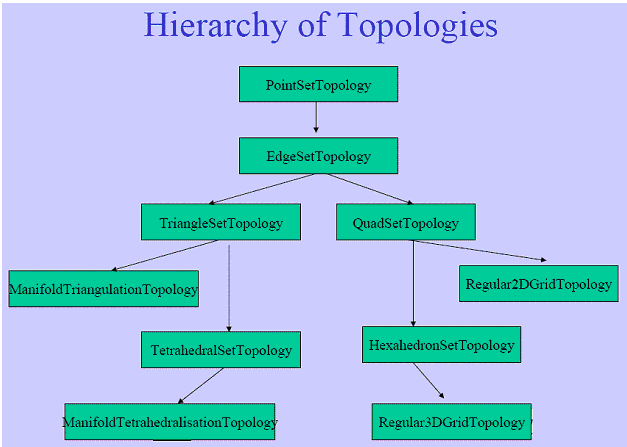
\includegraphics[width=0.95\linewidth]{Hierarchy_Topologies}
  \caption{A generic and hierarchical topology is described from a class called BaseTopology.}
 \label{fig:Hierarchy_Topologies}
\end{figure*}

BaseTopology class provides an implementation which handles
topological changes, full topological relationships and geometric
computation.

\subsubsection{How do I have access to the adjacency information between items ?}
\subsubsection{What to do if I need to know only basic topology information ?}
\subsubsection{What are the geometry algorithms stored in each topology classes ?}

\subsection{Handling Topological Changes}

\subsubsection{How does it work ?}
\subsubsection{What container should I use to handle the topology changes ?}
\subsubsection{How to write the different callback functions associated with the containers ?}

Topological changes are handled in a way which is as much
transparent for the user as possible.


\subsubsection{The 4 components of a BaseTopology object}

\begin{verbatim}

Class BaseTopology<DataTypes> {

// A container for info to be stored and methods to access adjacency :
//   - Adjacency Information is only computed when needed
//   - Non template class
//   - Store TopologicalChange list

TopologyContainer *container ;

// A modifier for low-level methods to change topology :
//   - Cannot be accessed from user
//   - Modifier also changes the DOFs in the Mechanical Object
//   - Low level methods to add or to remove an item
TopologyModifiers<DataTypes> *modifier ;

// TopologyAlgorithms for high-level methods to change topology (user access) :
//   - Accessed from the user
//   - High level algorithms to refine, cut mesh
TopologyAlgorithms<DataTypes> *topologyAlgorithms ;

// Geometry Algorithms methods to get geometry information :
//   - Compute geometric information (normal, curvature, area, length)
GeometryAlgorithms<DataTypes> *geometryAlgorithms ;

};

\end{verbatim}


\subsubsection{Implementation for objects inherited from each other (Point,
Edge, Triangle, Tetrahedron}


\begin{itemize}

 \item PointSetTopology (inherited from BaseTopology) :

    \begin{itemize}

    \item Container : For each point gives its global index. This is useful for subset topologies (subset triangulation, ...) where the number of vertices involved in the topology may not be the same as the total number of vertices.

    \item Modifier : addPointsProcess, removePointsProcess, renumberPointsProcess, addPointsWarning, removePointsWarning, propagateTopologicalChanges

    \item Geometry : computeCenter, computeRadius,
    getAABB()

    \end{itemize}


\item EdgeSetTopology (inherited from PointSetTopology)

    \begin{itemize}

    \item Container : array of edges, array of vertex-edge shell

    \item Modifier : addEdgesProcess, removeEdgesProcess, fuseEdgesProcess, splitEdgesProcess,
   addEdgesWarning, removeEdgesWarning

    \item Geometry : getEdgeLength, getRestEdgeLength

    \end{itemize}


\item TriangleSetTopology (inherited from EdgeSetTopology)

    \begin{itemize}

    \item Container : array of triangles, of vertex- and edge-triangle shell

    \item Modifier : addTrianglesProcess, removeTrianglesProcess, addTrianglesWarning, removeTrianglesWarning

    \item Topology Algorithms : InciseAlongPointsList, RemoveAlongTrianglesList

    \item Geometry : computeTriangleNormal

    \end{itemize}


\item TetrahedronSetTopology (inherited from TriangleSetTopology)

    \begin{itemize}

    \item Container : array of tetrahedra, array of vertex-, edge-, triangle-tetrahedra shell

    \item Modifier : addTetrahedraProcess, removeTetrahedraProcess, addTetrahedraWarning, removeTetrahedraWarning

    \item Geometry : computeTetrahedronVolume

    \end{itemize}

\end{itemize}

\begin{figure*}
 \centering
 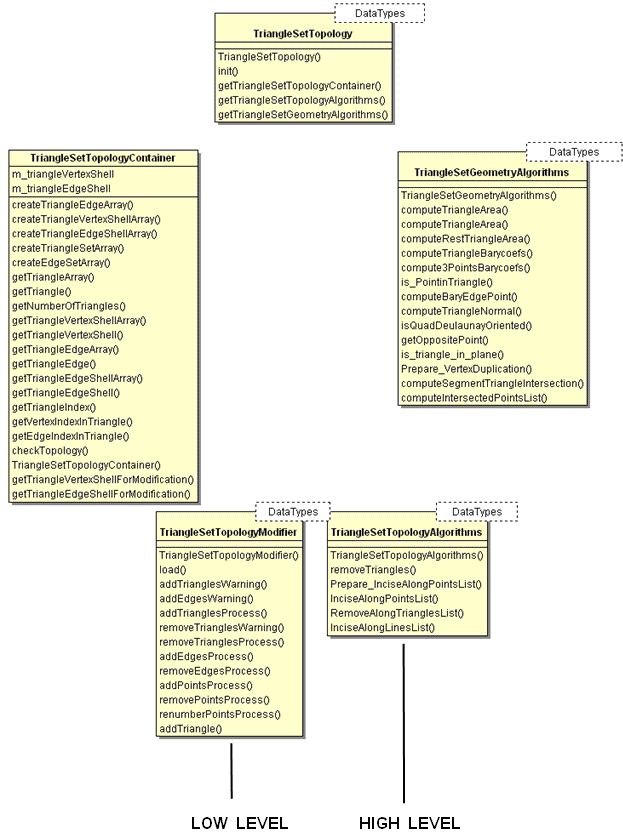
\includegraphics[width=0.95\linewidth]{UML_TriangleSetTopology}
  \caption{UML diagram describing the 4 components of TriangleSetTopology class.}
 \label{fig:UML_TriangleSetTopology}
\end{figure*}

\newpage

\begin{figure*}
 \centering
 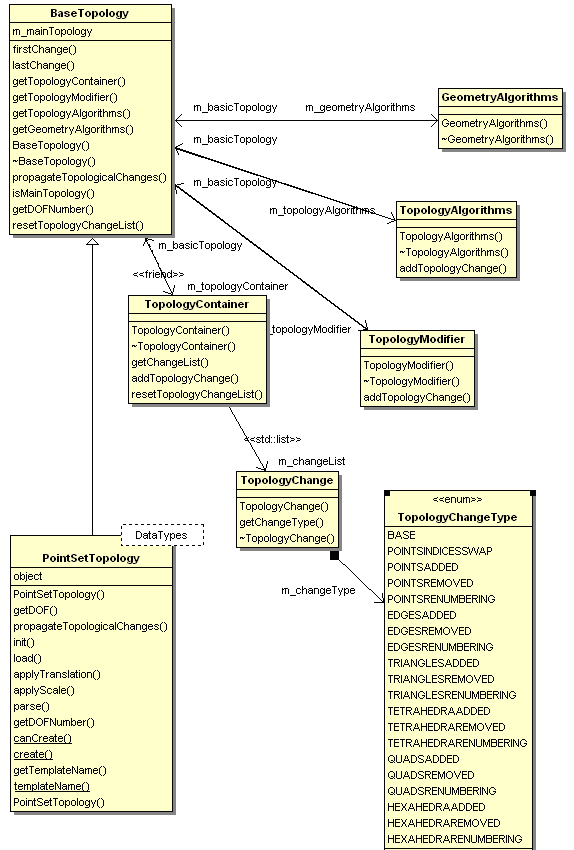
\includegraphics[width=0.95\linewidth]{UML_BaseTopology}
  \caption{UML diagram showing the use of a TopologyChanges List from BaseTopology class.}
 \label{fig:UML_BaseTopology}
\end{figure*}

\newpage

\subsubsection{Definition of data structures to be "aware" of topological
changes}

Force Fields, Constraints, Mapping and other modules may require to
store information for each topological item (point, edge, triangle,
etc.).
\\

Two container data structures are defined to handle topological
changes by matching the types of TopologyChanges :

\begin{itemize}

    \item PointData$<$MyType$>$, EdgeData$<$MyType$>$ are arrays (same as std::vector) of item of type MyType

    \item PointSubset, EdgeSubset are arrays of points or edges

\end{itemize}

Used-defined functions are called when an item is created or
destroyed.
\\

In higher level classes (for example
TriangularQuadraticSpringForceField, DiagonalMass or FixedConstraint
classes), the user only provides callback functions to handle :

\begin{itemize}

    \item the creation of a topological item
    \item the destruction of a topological item

\end{itemize}

\begin{figure*}
 \centering
 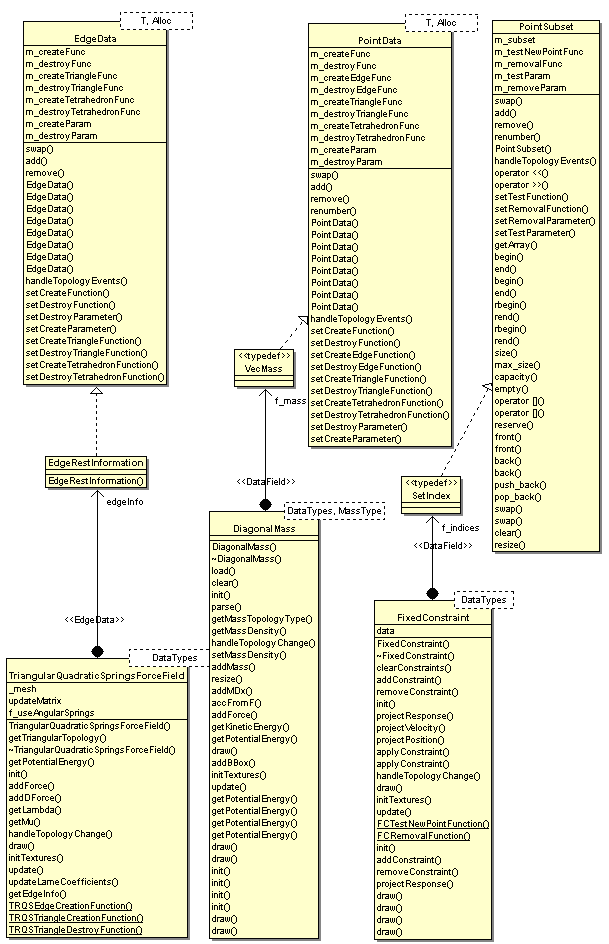
\includegraphics[width=0.95\linewidth, height=0.95\textheight]{UML_Topological_Changes}
  \caption{These UML diagrams show the use of EdgeData, PointData and
PointSubset to handle topological changes implying modifications
respectively in ForceField, Mass and Constraint modules.}
 \label{fig:UML_Topological_Changes}
\end{figure*}

\newpage

\begin{figure*}
 \centering
 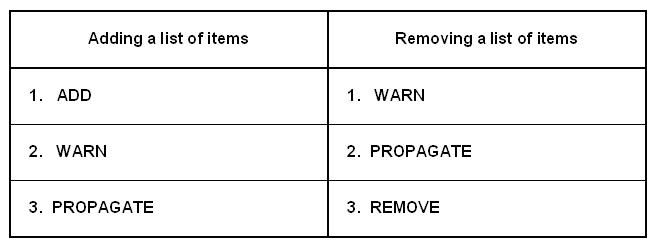
\includegraphics[width=0.95\linewidth]{Order_Notifications}
  \caption{Order to respect when adding or removing an item (see the
explanations in the following example).}
 \label{fig:Order_Notifications}
\end{figure*}

\begin{itemize}

    \item "WARN" means : add the current topological change (add or delete a list of items) in the list of TopologyChanges

    \item "PROPAGATE" means :  traverse the simulation tree with a TopologyChangeVistor to send
    the current topological change event to all force fields, constraints,
    mappings, etc.

\end{itemize}

\subsubsection{Example : What happens when I split an Edge ?}

\begin{figure*}
 \centering
 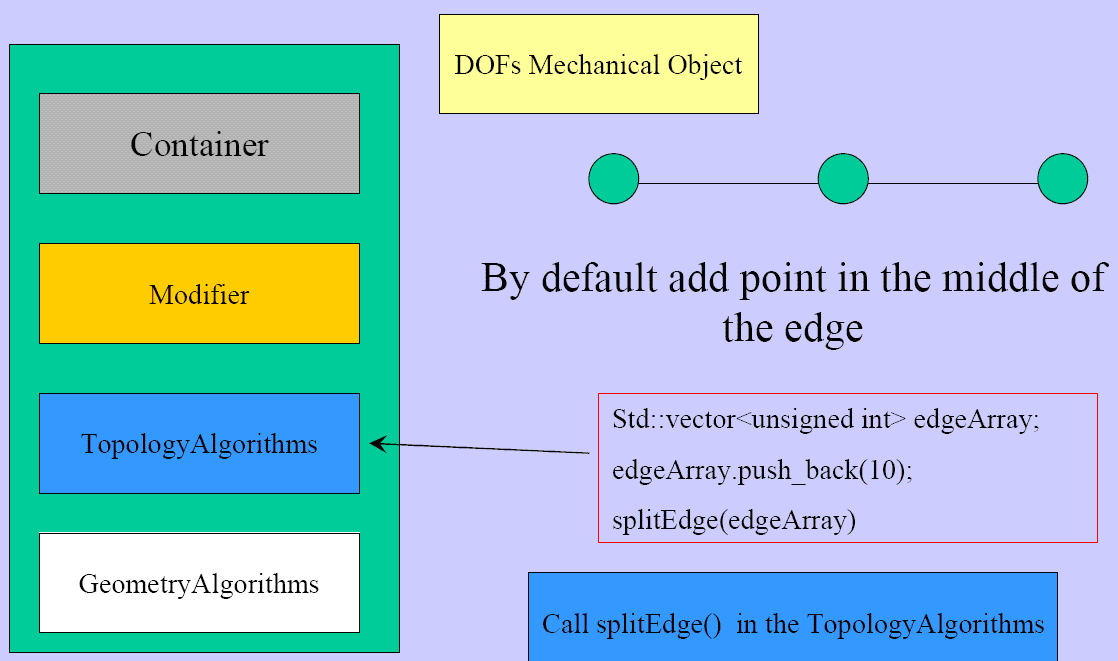
\includegraphics[width=0.95\linewidth]{Topology_Example_1}
 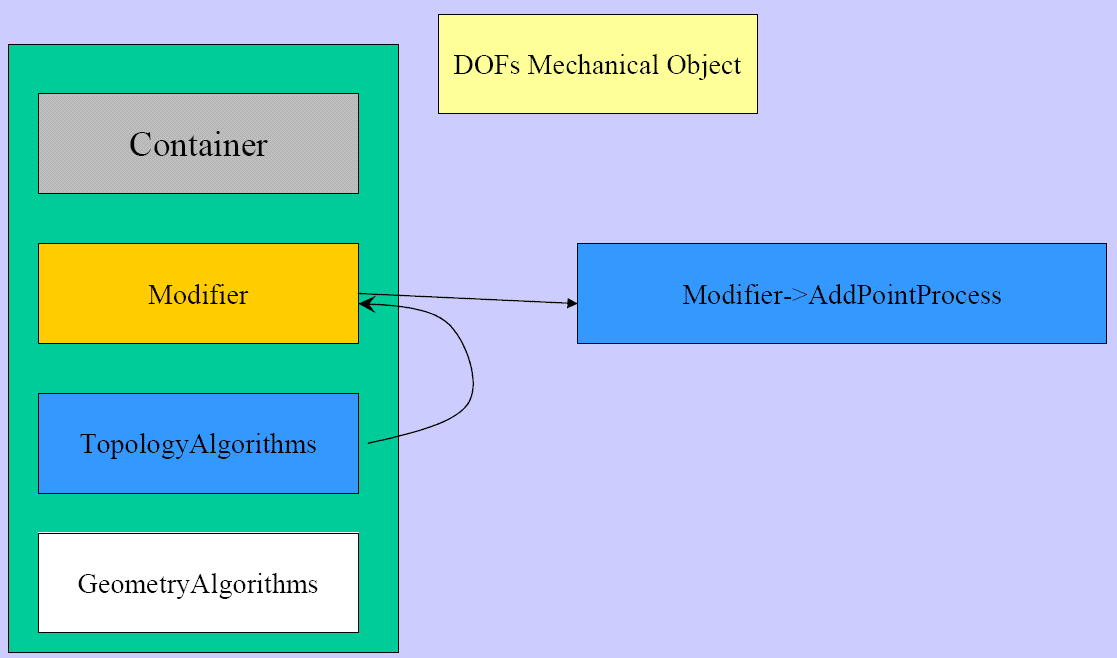
\includegraphics[width=0.95\linewidth]{Topology_Example_2}
  \caption{What happens when I split an Edge ? - Step 1. 2.}
 \label{fig:Topology_Example_12}
\end{figure*}

\newpage

\begin{figure*}
 \centering
 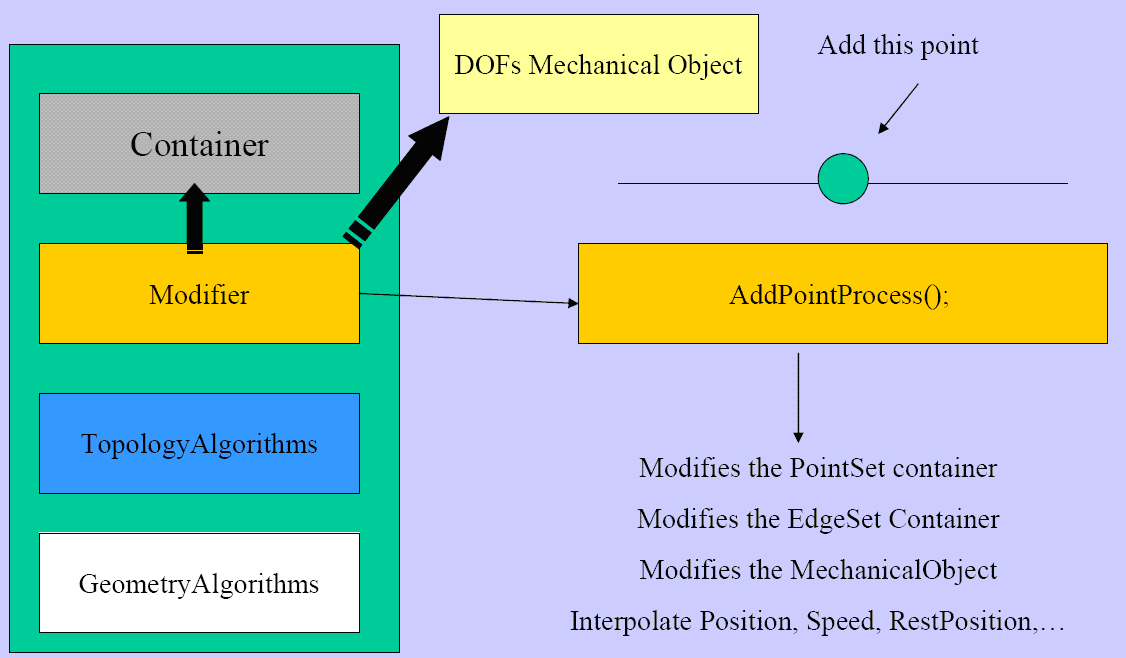
\includegraphics[width=0.95\linewidth]{Topology_Example_3}
 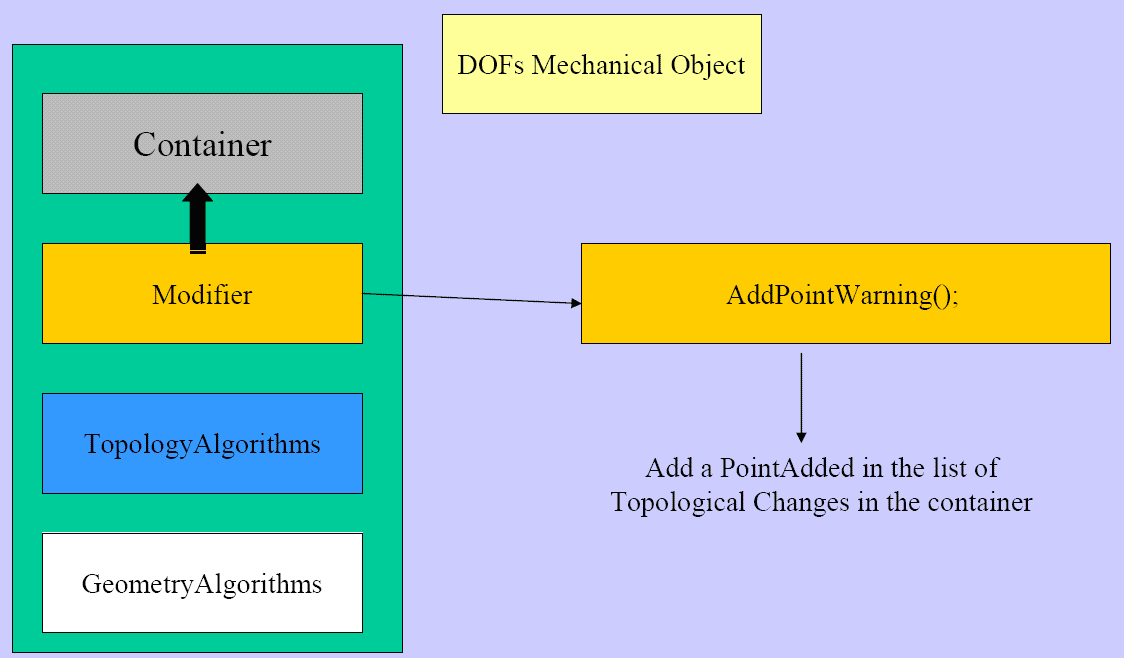
\includegraphics[width=0.95\linewidth]{Topology_Example_4}
  \caption{What happens when I split an Edge ? - Step 3. 4.}
 \label{fig:Topology_Example_34}
\end{figure*}

\newpage

\begin{figure*}
 \centering
 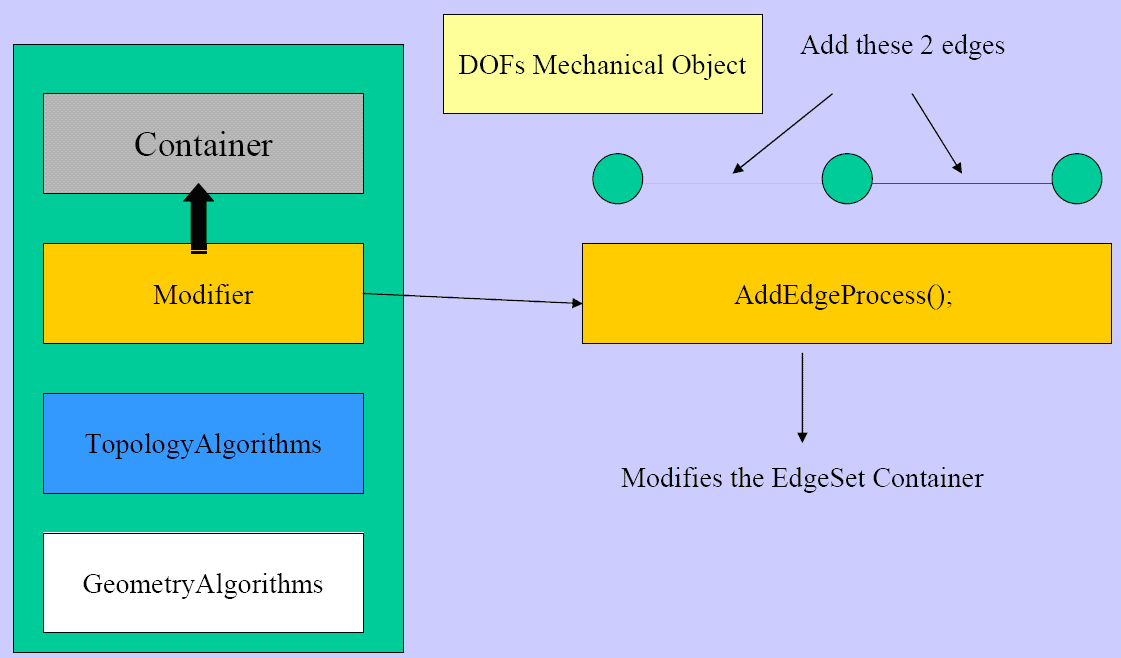
\includegraphics[width=0.95\linewidth]{Topology_Example_5}
 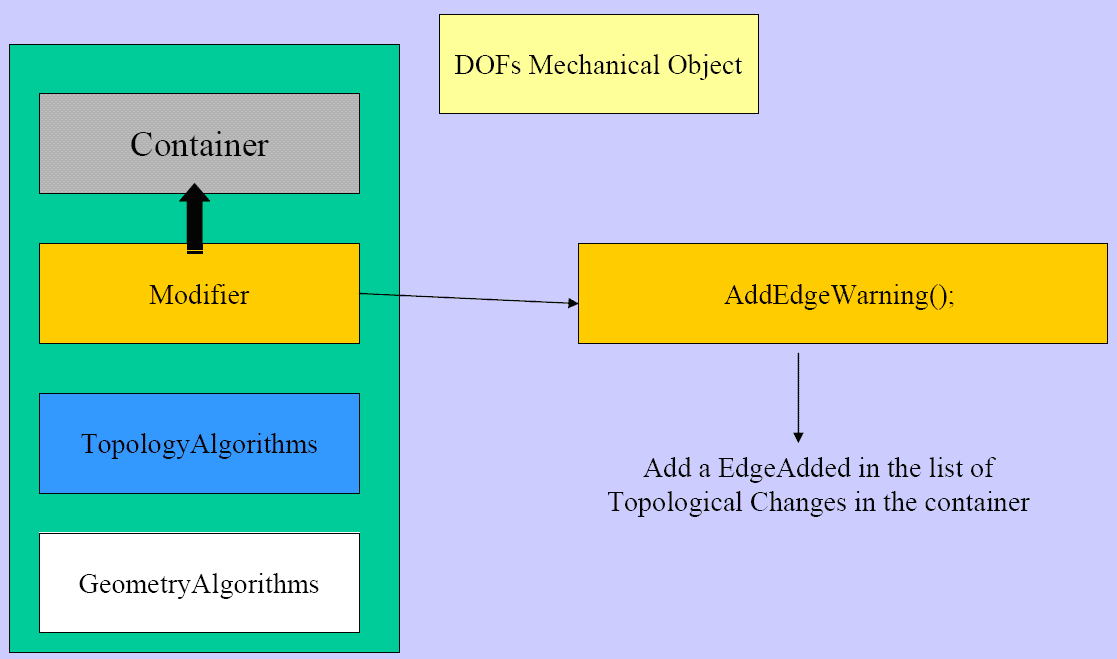
\includegraphics[width=0.95\linewidth]{Topology_Example_6}
  \caption{What happens when I split an Edge ? - Step 5. 6.}
 \label{fig:Topology_Example_56}
\end{figure*}

\newpage

\begin{figure*}
 \centering
 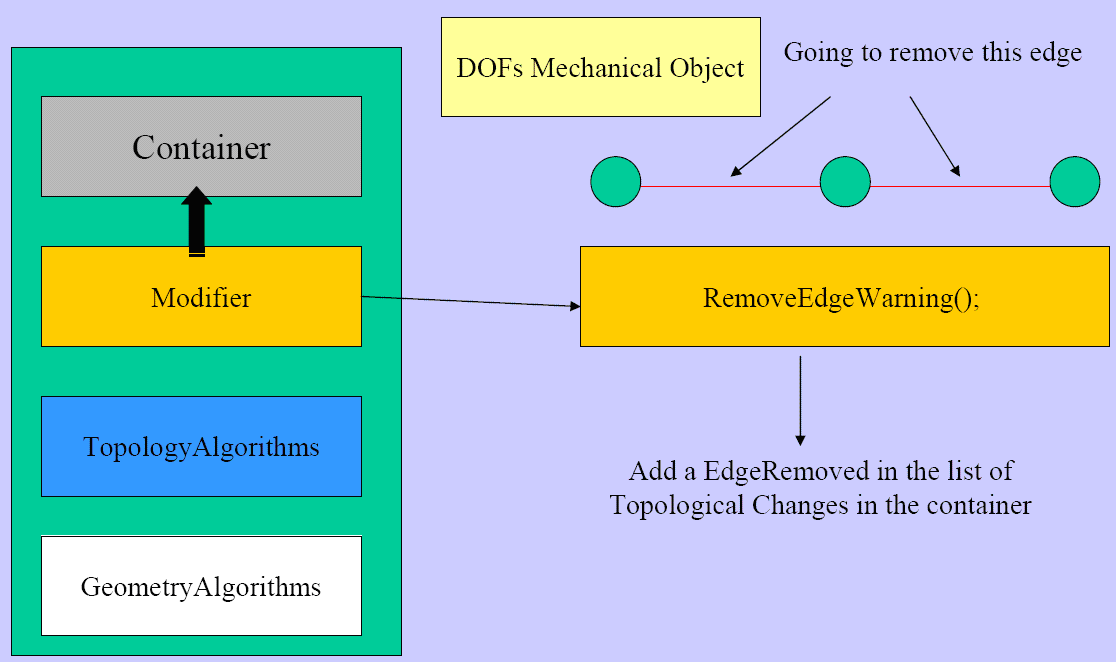
\includegraphics[width=0.95\linewidth]{Topology_Example_7}
 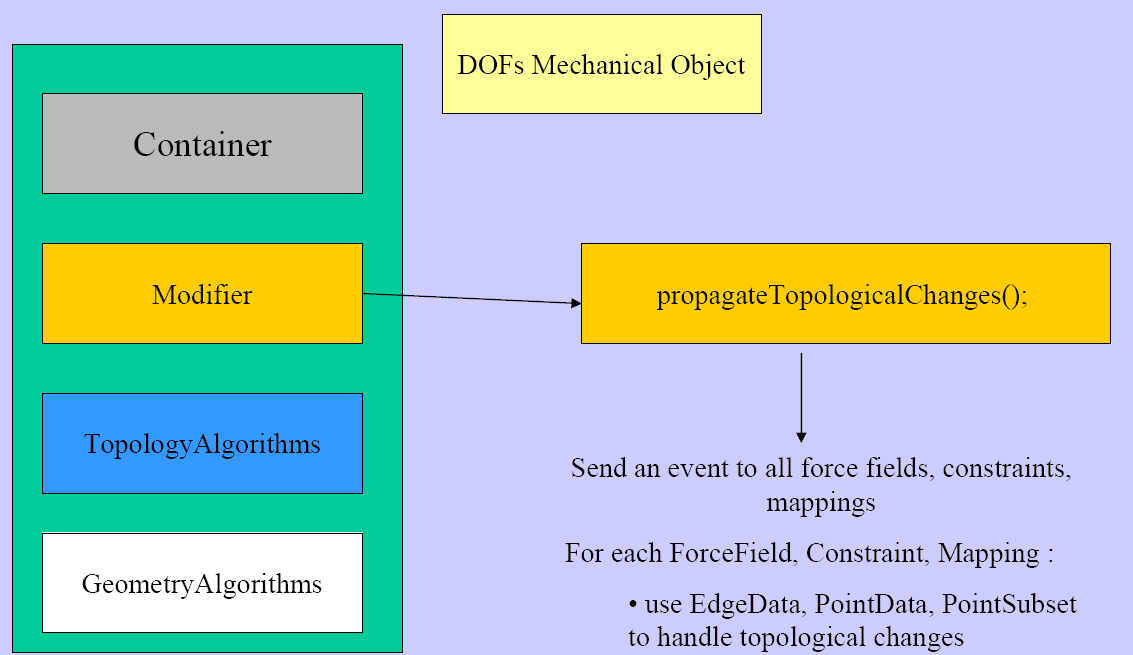
\includegraphics[width=0.95\linewidth]{Topology_Example_8}
  \caption{What happens when I split an Edge ? - Step 7. 8.}
 \label{fig:Topology_Example_78}
\end{figure*}

\newpage

\begin{figure*}
 \centering
 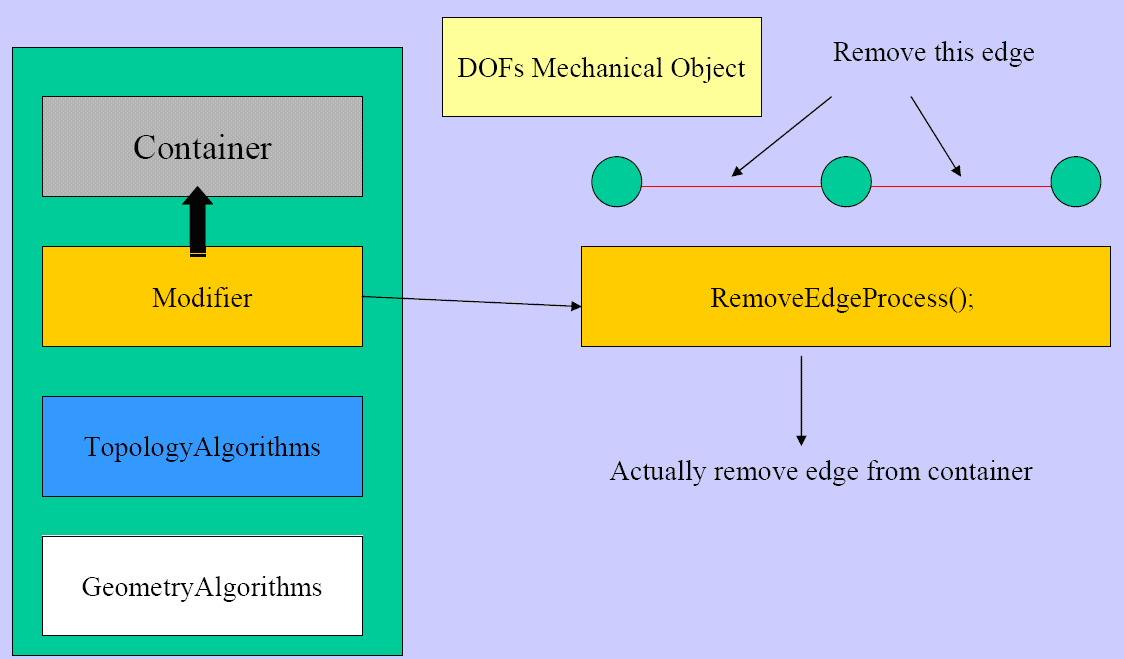
\includegraphics[width=0.95\linewidth]{Topology_Example_9}
  \caption{What happens when I split an Edge ? - Step 9.}
 \label{fig:Topology_Example_9}
\end{figure*}

\newpage

$ \ \ $

\newpage

\subsection{Designing Topological Mappings}

\subsubsection{What is a Topological Mapping ?}

A TopologicalMapping is a new kind of Mapping which converts an
input topology to an output topology (both topologies are of type
BaseTopology).
\\

It first initializes the mesh of the output topology from the mesh
of the input topology, and it creates the two Index Maps that
maintain the correspondence between the indices of their common
elements.
\\

Then, at each propagation of topological changes, it translates the
topological change events that are propagated from the input
topology into specific actions that call element adding methods or
element removal methods on the output topology, and it updates the
Index Maps.
\\

So, at each time step, the geometrical and adjacency information are
consistent in both topologies.


\subsubsection{Example : from TetrahedronSetTopology to TriangleSetTopology}

Here is the scene-graph corresponding to the simulation of an object
which can be represented as a tetrahedral volume (on which one
volume force is applied) or as a triangular surface (on which two
surface forces are applied). Note that the Visual Model and the
Collsion Model are attached to the surface mesh of the object :


\begin{figure*}
 \centering
 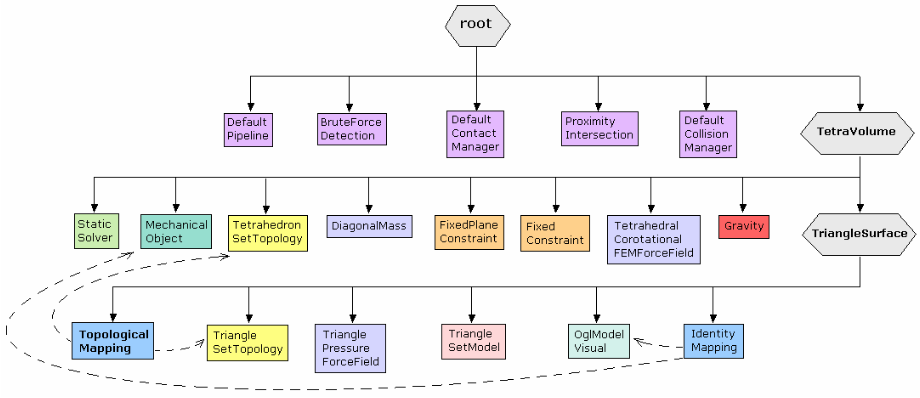
\includegraphics[width=1.0\linewidth]{Scene_Graph_TopologicalMapping}
  \caption{Scene Graph illustrating a TopologicalMapping from a TetrahedronSetTopology to a TriangleSetTopology.}
 \label{fig:Scene_Graph_TopologicalMapping}
\end{figure*}


% \subsubsection{Use Cases}
